\chapter{Signed scripture corpora: the Qur'an and the hadith}
\label{sec:scripture}

The lexicons of Chapter~\ref{sec:lexicons} hold single signs. This chapter describes the continuous signing of whole
ayat and hadith by human signers: five Qur'an datasets and a new signed hadith corpus, how each sample was labelled,
what the data contain, and the quality problems we found in all of them and corrected. Every figure comes from the
published builds and the pipeline state of 6 October 2026, computed by \code{docs/paper/tools/scripture\_eda.py}. The
hadith corpus was still growing on that date; the figures are a snapshot.

\section{Five signed Qur'an datasets}
\label{sec:quran_sets}

Table~\ref{tab:quran_sets} lists the five Qur'an datasets now published, two more than Section~\ref{sec:lexicons}
described. For the three YouTube sources (King Fahd Complex, al-Mukhtasar fi Tafsir, Al-Kharj curriculum), Whisper
\cite{whisper} supplies only the timing; each segment's label is the fixed Uthmani text, aligned to the timed
transcript, so a recognition error never becomes a label. Tebyan\footnote{Tebyan Qur'an: \url{https://tebyanquran.com}}
publishes one clip per ayah (some clips cover several), so its labels are the publisher's own. Diyanet's two Qur'an
episodes in Turkish Sign Language\footnote{Diyanet \.{I}\c{s}leri Ba\c{s}kanl\i\u{g}\i, ``\.{I}\c{s}aret Dili ile
Kur'an'', YouTube playlist PLtApkPE49w-tQ8-zFm1QVrwrmYKauonS9.} gave a false alignment, because Whisper caught the
spoken basmala of the introduction; their labels come from the text panels the publisher shows while each phrase is
signed.

\begin{table}[ht]
\centering
\small
\caption{The five signed Qur'an datasets as published (private Hugging Face datasets). A segment is one ayah's recitation or one passage of tafsir; hours are the signed time.}
\label{tab:quran_sets}
\begin{tabular}{llrrrrrr}
\toprule
Source & SL & Segments & Recitation & Tafsir & Ayahs & Surahs & Hours \\
\midrule
King Fahd Complex & ArSL & 1,066 & 592 & 468 & 558 & 38 & 7.4 \\
al-Mukhtasar fi Tafsir & ArSL & 6,127 & 0 & 6,092 & 5,916 & 112 & 34.7 \\
Al-Kharj curriculum & ArSL & 207 & 207 & 0 & 186 & 22 & 0.3 \\
Tebyan & ArSL & 567 & 567 & 0 & 570 & 38 & 2.4 \\
Diyanet & TİD & 13 & 13 & 0 & 12 & 2 & 0.1 \\
\bottomrule
\end{tabular}
\end{table}


Together the five datasets hold 7,980 labelled segments and about 44.9 hours of signing. Al-Mukhtasar alone covers 5,916
ayat of 112 surahs, almost all as tafsir: the signer explains each ayah rather than reciting it. Each dataset is a
private Hugging Face repository with a manifest (one row per segment, with its YouTube timestamp), the full MediaPipe
Holistic keypoints and the same motion as Isharati poses; no video is redistributed. In the application each ayah can
be played by any of the signers that cover it (Section~\ref{sec:scripture_app}).

\section{A signed hadith corpus}
\label{sec:hadith_corpus}

Section~\ref{sec:intro} motivated Isharati partly by the absence of a hadith collection in sign language. That claim
needs a correction: signed hadith exist, in some quantity, on YouTube, made by Deaf associations and educational
channels. What does not exist is a collection that can be searched, aligned to the hadith text or used to train and
drive a signing model. We built one.

\subsection{Sources}
A search of YouTube for hadith in sign language (Arabic and Turkish queries) found 14 sources: playlists and channels
of Islamweb for Deaf\footnote{\url{https://www.youtube.com/channel/UCf61i7CZLHYBSm3wz7dY_yg}}, the Insan association's
Nawawi's Forty in sign language, the Deaf Educational Channel\footnote{\url{https://www.youtube.com/channel/UC86B8NmyJ4n4PkUhLpkAP9Q}}
(Umdat al-Ahkam, Riyad al-Salihin, thirty hadith for women and a Nawawi series), three Deaf preachers' Nawawi lessons,
and two Turkish sources (``\.{I}\c{s}aret Dili ile 40 Hadis''). In all, 824 videos and 114.4 hours. They come in two
kinds: \emph{clips}, one hadith per video, often under five minutes, and \emph{lessons}, a signed explanation of one
hadith that can last an hour. Videos are streamed: each is downloaded, transcribed, matched and reduced to keypoints, and
then deleted, so the corpus keeps only keypoints and links.

\subsection{Labelling: the label is always the collection's text}
\label{sec:hadith_labels}
A label is a hadith as printed in its collection, taken from the open hadith-api \cite{hadithapi} (Bukhari, Muslim, Abu
Dawud, Tirmidhi, Nasa'i, Ibn Majah, Malik, Nawawi's Forty and the Qudsi hadith, in Arabic, English and Turkish). A
transcript or an on-screen text only says \emph{which} hadith a video signs; it never becomes the label. Four routes lead
to a label, chosen by what the video offers:

\begin{enumerate}[leftmargin=*,itemsep=2pt]
  \item \textbf{Voice-over.} Where an interpreter reads the hadith aloud, a local Whisper large-v3-turbo model gives word
        timestamps, and the transcript is matched word by word against the collections (a word-bigram index weighted by
        inverse document frequency proposes candidates; an ordered alignment confirms them). A match needs at least
        8 words in order, at least 55\% of the transcript words inside the span, and at least 3 distinctive word pairs.
        The last condition was added after a chain of narrators alone (``\ar{عن أبي هريرة رضي الله عنه قال قال رسول الله}'')
        matched dozens of unrelated hadith. The span where the text is read is kept as \code{read\_start}, \code{read\_end}.
  \item \textbf{Translation.} The Turkish voice-overs paraphrase a translation, so word matching fails. A language model
        names the Arabic hadith and the time span, and the Arabic collections must confirm the proposed text, or the
        proposal is dropped.
  \item \textbf{On-screen text.} 450 of the 638 videos transcribed so far (71\%) are silent or carry only room noise:
        Deaf-made content often has no voice. Most show the hadith on screen, so a vision model reads the text from a
        few frames and the collections confirm it. The model matters: a smaller model, given a decorative font, returned
        the text of a famous hadith instead of the one on screen, which the collections then confirmed. A larger model
        read it correctly, and every such label is cross-checked against the hadith number in the title; a disagreement
        is flagged, not resolved silently.
  \item \textbf{Title.} A silent clip whose screen cannot be read keeps the publisher's number from its title (for
        Nawawi's Forty, the text follows from the number). An early parser read ``\ar{الحديث الثاني | الأربعون النووية}''
        as hadith 42; the fixed parser stops at the separator, and 31 title references were corrected.
\end{enumerate}

\subsection{Keypoints and the signer's face}
Each sample is a whole clip, trimmed to the frames in which the signer is visible, or, in a voiced lesson, the span
where a hadith is read. MediaPipe Holistic \cite{mediapipeholistic} gives pose, hands and the 478-point face mesh for
every frame; the same pass now also keeps the 52 face blendshape scores (brows, eyes, mouth), so the avatar can carry
the signer's facial expression and the skeleton view can draw the face. The face is published as 160 contour points on
the same 25\,fps frames as the Isharati pose, centred on the neck and in shoulder widths like the body.

\subsection{What the corpus contains}
\begin{table}[ht]
\centering
\small
\caption{Signed hadith samples per source in the published snapshot (6 October 2026). Labelled samples carry a hadith verified against its collection; hours are the signed time after trimming.}
\label{tab:hadith_sources}
\begin{tabular}{llrrrr}
\toprule
Source & SL & Samples & Labelled & Distinct hadith & Hours \\
\midrule
Deaf Educational Ch., Umdat al-Ahkam & ArSL & 134 & 129 & 128 & 6.55 \\
Islamweb for Deaf & ArSL & 103 & 95 & 59 & 3.91 \\
Insan, Nawawi's Forty & ArSL & 52 & 50 & 50 & 1.03 \\
Deaf Educational Ch., Riyad & ArSL & 26 & 19 & 19 & 1.20 \\
H. Wadwid, hadith & ArSL & 24 & 8 & 8 & 0.98 \\
E. Demir, 40 Hadis (TİD) & TİD & 23 & 18 & 17 & 0.07 \\
Deaf Educational Ch., 30 for women & ArSL & 19 & 15 & 15 & 1.18 \\
M. Hafez, Nawawi's Forty & ArSL & 15 & 15 & 15 & 0.26 \\
TİD, single videos & TİD & 5 & 0 & 0 & 0.14 \\
ArSL, single videos & ArSL & 3 & 2 & 2 & 0.04 \\
\midrule
Total & & 404 & 351 & 282 & 15.37 \\
\bottomrule
\end{tabular}
\end{table}


\begin{figure}[ht]
\centering
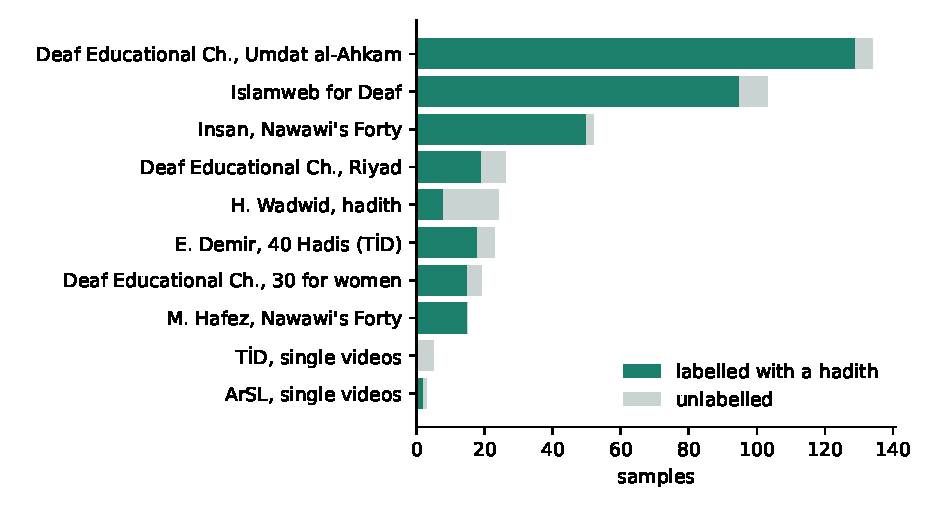
\includegraphics[width=0.92\textwidth]{figures/hadith_sources.pdf}
\caption{Signed hadith samples per source in the published snapshot. The grey part of each bar has no verified label
(it is hidden in the application).}
\label{fig:hadith_sources}
\end{figure}

The snapshot holds 404 samples and 15.4 hours of signing. 351 samples (87\%) carry a verified hadith, 333 in ArSL and
18 in T\.{I}D, covering 282 distinct hadith. The routes of Section~\ref{sec:hadith_labels} contributed 185 labels from
on-screen text, 146 from voice-overs, 18 from translations and 2 from titles alone; for 218 labels the publisher's
title agrees with the text match. Figure~\ref{fig:hadith_collections} shows where the labels come from: Bukhari (133)
and Muslim (69) dominate, as the sources teach the canonical hadith, and Nawawi's Forty is complete but for one
hadith (41 of 42). Most hadith have one signer (229); 53 have two to five, which is what a comparison between signers
needs. The signer is detected in 88\% of frames, the hands in 62\% (a hand at rest is often outside the frame), the face
in 79\%; 364 samples carry the blendshape scores.

\begin{figure}[ht]
\centering
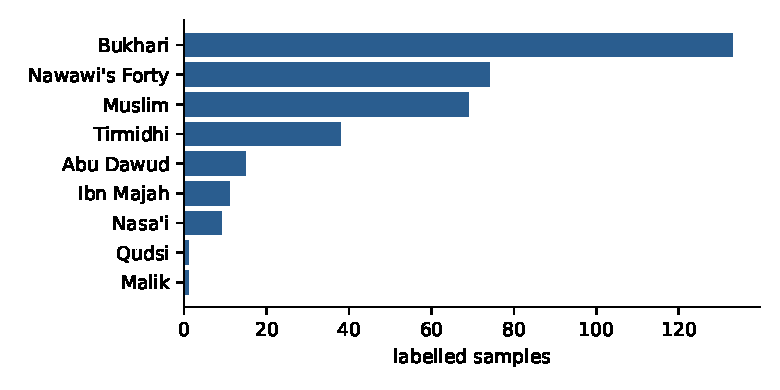
\includegraphics[width=0.72\textwidth]{figures/hadith_collections.pdf}
\caption{Collection of each verified hadith label. A hadith in several collections is counted once, under the collection
whose text matched best (Nawawi's Forty first for the Nawawi series).}
\label{fig:hadith_collections}
\end{figure}

Four lesson series (65.7 hours) are listed but not yet in the snapshot. The two transcribed so far are silent, so they
need the on-screen route, and a lesson yields one sample per hadith rather than per video.

\subsection{Gloss targets}
Each hadith also gets a sentence-level gloss, made by the application's own lexicon-constrained glossers (ArSL for the
Arabic text, T\.{I}D for the Turkish translation). The glosser is given the Prophet's words only: the chain of narrators
and the source note (``\ar{رواه البخاري}'') are cut first, a step that needed two fixes (an HTML line break before the
source note, and hadith in which a companion asks a question and no ``\ar{قال رسول الله}'' marks the start). Of the 206
ArSL glosses, the median share of words with no recorded sign is 33\%; of the 12 T\.{I}D glosses, 7\%. These glosses
are a text-to-sign target, not an annotation of what the human signer did: the signer's own choice and order of signs
differ, and a gloss is shown in the application only under a signer of the same sign language.

\section{Pose quality across all signed datasets}
\label{sec:pose_qa}

A visual check of the hadith samples in the application found skeletons that looked stretched, and an avatar whose arm
folded into its face. An automatic check of every published sample (\code{scripts/eval/qa\_sign\_datasets.py}: body
proportions, joint jumps, hand-to-wrist distance, face alignment, labels and glosses) showed that the problem was not
limited to the hadith.

\paragraph{Square units.} MediaPipe returns $x$ as a share of the frame's width and $y$ as a share of its height. On a
16:9 video one unit of $x$ is 1.78 units of $y$, so a pose normalised by shoulder width came out stretched tall: the
upper arm measured 1.25--1.44 shoulder widths, where an adult's is about 0.7--0.9. Every published pose is now built
from $x \cdot w/h$, with $w/h$ taken from each video (the clip's metadata, or the downloader's record of the
downloaded format), and a pose whose frame size is unknown is refused rather than published stretched.

\paragraph{Glitches and wrong figures.} A joint that sits more than 0.5 shoulder widths from the median of its seven
neighbouring frames is blanked and interpolated (real signing does not move a wrist that far and back within a few
frames). Frames whose shoulder width is far from the clip's own (0.6--1.6 times the median) are dropped at the ends of
a clip and interpolated inside it: they were introduction and closing cards in which a small figure, or a book cover,
was detected instead of the signer.

\begin{table}[ht]
\centering
\small
\caption{Pose quality before and after the two corrections, on a random sample of clips per dataset. Upper arm over shoulder width is about 0.7--0.9 in adults; a jump is a body joint moving more than 0.6 shoulder widths between two frames at 25\,fps.}
\label{tab:pose_qa}
\begin{tabular}{lrrrrr}
\toprule
& & \multicolumn{2}{c}{Upper arm / shoulder} & \multicolumn{2}{c}{Jumps per 100 frames} \\
\cmidrule(lr){3-4}\cmidrule(lr){5-6}
Dataset & Clips & raw units & square units & before filter & after filter \\
\midrule
King Fahd Complex & 60 & 1.41 & 0.87 & 0.19 & 0.10 \\
al-Mukhtasar fi Tafsir & 60 & 1.42 & 0.86 & 0.13 & 0.04 \\
Al-Kharj curriculum & 60 & 1.29 & 0.81 & 0.05 & 0.05 \\
Tebyan & 60 & 1.39 & 0.84 & 0.41 & 0.21 \\
Diyanet & 13 & 1.25 & 0.77 & 0.01 & 0.00 \\
Signed hadith & 120 & 1.32 & 0.83 & 2.96 & 1.75 \\
\bottomrule
\end{tabular}
\end{table}


\begin{figure}[ht]
\centering
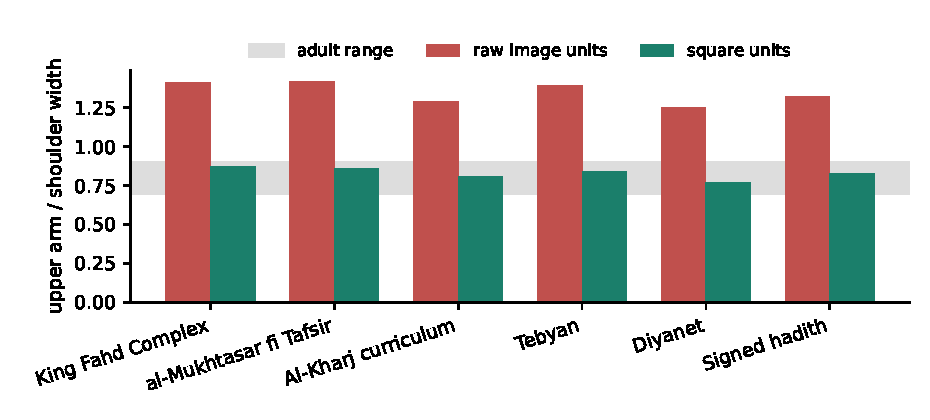
\includegraphics[width=0.92\textwidth]{figures/pose_aspect_qa.pdf}
\caption{Upper arm over shoulder width, median over a random sample of clips per dataset, in raw image units and in
square units. The grey band is the adult range.}
\label{fig:pose_aspect_qa}
\end{figure}

Table~\ref{tab:pose_qa} and Figure~\ref{fig:pose_aspect_qa} show the effect on a random sample of each dataset: every
dataset moves into the adult range (0.77--0.87), and the spike filter halves the joint jumps where they were frequent
(hadith 2.96 to 1.75 per 100 frames, Tebyan 0.41 to 0.21). Over every published sample, the upper arm was out of
the adult range in 1,036 of 1,066 King Fahd segments, 550 of 567 Tebyan, 203 of 207 Al-Kharj and all 13 Diyanet
segments before the correction, and in 4 King Fahd segments after it. What the check still flags is mostly motion,
not shape: joint jumps in 133 of the 404 hadith samples (most in the seated Umdat al-Ahkam lessons, where the
sheikh turns and leans) and in under 1\% of the Qur'an segments; a hand drifting from its wrist in 16 hadith samples,
126 King Fahd, 56 Tebyan and 171 of the 6,127 al-Mukhtasar segments.

\paragraph{The lexicon had the same bias.} The lexicon does not keep each video's aspect, but it already rescaled every
sign to one body shape (Section~\ref{sec:lexicons}): the nose-to-neck height over shoulder width was set to 0.74, the
median of ASL Citizen. That median was measured on 4:3 webcam frames, so every lexicon sign was normalised to a body
about 1.5 times too tall. In square units the five datasets above give 0.47--0.55; the lexicon reference is now 0.50.

\section{Retargeting to realistic avatars}
\label{sec:retarget_realistic}
The realistic avatars (Rocketbox, Section~\ref{sec:avatars}) did not bend their elbows in signs that need it. On
\ar{وضوء} (KArSL sign 0381), the signer's right elbow is at 104\textdegree{} (180\textdegree{} is straight), the cartoon
avatar's at 90\textdegree{}, and the Rocketbox avatars' at 148\textdegree{} (women) and 178\textdegree{} (men). The cause
is reach. Hand targets are placed on the avatar's body in the signer's shoulder widths; the Rocketbox arms are 1.3--1.4
shoulder widths long against the cartoon's 2.0, so in 29 of the sign's 38 frames the target lay beyond a man's arm, and
a two-bone inverse kinematics solver reaches an unreachable point with a straight arm.

The solver now limits the distance from shoulder to wrist to what the avatar's own arm reaches with the signer's elbow
angle $\theta$: $d \le \sqrt{L_1^2 + L_2^2 - 2 L_1 L_2 \cos\theta}$, with $L_1$, $L_2$ the avatar's upper arm and
forearm. A reachable target is unchanged, and so is a target at the face, where the contact carries the meaning. After
this change and the lexicon correction above, the Rocketbox elbows on \ar{وضوء} are within 0.3--4.1\textdegree{} of the
signer's (Table~\ref{tab:retarget_realistic}). The cartoon's longer arms now bend more than the signer's
(88\textdegree{} against 122\textdegree{}): with arms that long, the hand cannot be in the right place and the elbow at
the signer's angle at the same time, and we keep the hand.

\begin{table}[ht]
\centering
\small
\caption{Avatar retargeting before and after the corrections (\code{scripts/avatars/retarget\_eval.py}, 15 signs, 21
hand tracks; \code{elbow\_eval.py} for \ar{وضوء}). Height error is in nose heights, side error in shoulder widths, elbow
angles in degrees for the right arm (signer: 104\textdegree{} in the old body shape, 122\textdegree{} in the corrected one).}
\label{tab:retarget_realistic}
\begin{tabular}{lrrrr}
\toprule
& Height error & Side error & Palm flipped & Right elbow \\
\midrule
Cartoon, before & 0.09 & 0.04 & 1\% & 90 \\
Cartoon, after & 0.08 & 0.03 & 0\% & 88 \\
Rocketbox man, before & 0.15 & 0.06 & 0\% & 178 \\
Rocketbox man, after & 0.15 & 0.06 & 0\% & 123 \\
\bottomrule
\end{tabular}
\end{table}

\section{Where the corpora appear in the application}
\label{sec:scripture_app}
The application now has one page for each scripture: the Sign Mushaf (\code{\#/quran}) and Signed Hadith
(\code{\#/hadith}), reachable from a menu that lists pages only (home, Academy, Qur'an, hadith and the review studio).
The Academy groups them by sign language: a learner choosing ArSL sees the Qur'an and hadith cards with the ArSL
signers, a T\.{I}D learner the Diyanet Qur'an and the Turkish hadith, and a language with no such data shows neither.
The hadith page lists hadith by collection, Nawawi's Forty first; a hadith shows its Arabic text and translation, one
chip per signer, the avatar or skeleton replaying that signer's keypoints with the face, a jump to where the text is
read, the original video at its timestamp, and the gloss with the words that have no recorded sign in red. The landing
page keeps a short preview of both. The data are read from the private datasets at start-up and re-read every 30
minutes, so a new sample appears without redeploying.

\section{Limitations of the scripture corpora}
\begin{itemize}[leftmargin=*,itemsep=2pt]
  \item The videos state no licence. The datasets are private and hold links and keypoints only; permission is to be
        requested from every publisher before any release.
  \item A hadith label says which hadith a video signs, not that the signing is a faithful rendering of its text. The
        translation and on-screen routes depend on a language or vision model whose proposal the collections must
        confirm; a confirmed but wrong proposal (a famous hadith read in place of the one on screen) remains possible
        where the title gives no number to check against.
  \item Labels mark the whole clip, not each sign. Sign-level alignment inside a hadith, and a Deaf reviewer's check of
        the labels, are still to do.
  \item 53 samples (13\%) have no label, and the joint-jump and detached-hand flags of Table~\ref{tab:pose_qa} remain in
        the seated lessons, where much of the movement is the signer turning in his seat.
  \item The corpus is not balanced: two sources (Islamweb for Deaf and the Deaf Educational Channel's Umdat al-Ahkam)
        supply more than half of the samples, and T\.{I}D has 18 labelled samples.
\end{itemize}
